\documentclass[11pt,a4paper]{article}
\usepackage[utf8]{inputenc}
\usepackage[T1]{fontenc}
\usepackage{amsmath,amssymb}
\usepackage{graphicx}
\usepackage{hyperref}
\usepackage{geometry}
\usepackage{booktabs}
\usepackage{caption}
\usepackage{subcaption}
\usepackage{xcolor}
\usepackage{tikz}
\usepackage{pgfplots}
\usepackage{setspace}
\pgfplotsset{compat=1.18}
\usetikzlibrary{arrows.meta,positioning,shapes.geometric,fit,backgrounds,calc}

% Wong color-blind friendly palette (Saloni's guidelines)
\definecolor{cbBlue}{HTML}{0072B2}
\definecolor{cbVermillion}{HTML}{D55E00}
\definecolor{cbGreen}{HTML}{009E73}
\definecolor{cbPurple}{HTML}{CC79A7}
\definecolor{cbOrange}{HTML}{E69F00}
\definecolor{cbSkyBlue}{HTML}{56B4E9}
\definecolor{cbYellow}{HTML}{F0E442}
\definecolor{cbBlack}{HTML}{000000}
\definecolor{hypothesisbg}{HTML}{FFF8E1}

\geometry{left=2.5cm,right=2.5cm,top=2.5cm,bottom=2.5cm}
\onehalfspacing

\title{\textbf{Targeting the NME2-MYC Transcriptional Axis:\\Structural Insights from NDPK Hexamer Dynamics\\and Implications for Stauprimide-Based Therapeutics}}
\author{Ashish (tp53)\thanks{Correspondence: acgt0101@gmail.com}}
\date{February 2026}

\begin{document}

\maketitle

\begin{abstract}
\noindent
The MYC oncogene is dysregulated in approximately 75\% of human cancers, yet it remains largely refractory to direct pharmacological intervention due to its intrinsically disordered structure. The small molecule stauprimide offers an indirect strategy: it binds nucleoside diphosphate kinase B (NME2/NDPK-B), a transcription factor that activates MYC expression by resolving G-quadruplex structures in the MYC promoter, and prevents its nuclear translocation. Stauprimide selectively suppresses MYC transcription across diverse cancer cell lines (EC$_{50}$ 30~nM--8~$\mu$M) and inhibits tumor growth in xenograft models, yet the structural basis for its selectivity for NME2 over the 88\%-identical NME1 isoform remains unknown. Recent computational studies on NDPK hexamer dynamics have revealed that NME1-NME2 heterohexamers, particularly the A$_1$B$_5$ configuration (one NME1, five NME2 subunits), represent the most thermodynamically stable nuclear-competent species. These studies further identified the C-terminal tail and Kpn loop interface as critical determinants of hexamer stability, and showed that the approximately 18 residues differing between NME1 and NME2 are located outside the hexameric interface. In this perspective, we integrate these structural dynamics findings with the established pharmacology of stauprimide to propose a testable hypothesis: stauprimide selectively disrupts A$_1$B$_5$ heterohexamer assembly by binding NME2 at or near its isoform-specific surface residues, perturbing the Kpn loop--C-terminal interface required for nuclear-competent oligomerization. We discuss the clinical implications of this mechanism in the context of NME2-MYC axis activation in enzalutamide-resistant prostate cancer and outline the experimental validations required to advance NME2-targeting therapeutics.
\end{abstract}

\section{Introduction}

The MYC proto-oncogene encodes a master transcription factor that governs cell proliferation, metabolism, and apoptosis. Its overexpression or dysregulation is observed in up to 75\% of all human cancers, correlating with aggressive disease, poor prognosis, and treatment resistance across tissue types~\cite{casey2016}. Beyond its direct roles in tumor cell biology, MYC also modulates the tumor microenvironment through regulation of immune checkpoint molecules CD47 and PD-L1, enabling immune evasion~\cite{casey2016}. Genetic studies in transgenic mouse models have demonstrated that MYC inactivation can induce tumor regression, establishing it as a validated therapeutic target~\cite{bouvard2017}. Nevertheless, MYC has proven exceptionally difficult to drug directly: it lacks well-defined binding pockets, functions through protein--protein interactions with its obligate partner MAX, and its intrinsically disordered regions resist conventional small-molecule approaches.

Several indirect strategies for suppressing MYC have been explored. Bromodomain and extraterminal domain (BET) inhibitors such as JQ1 reduce MYC transcription by disrupting epigenetic activation at superenhancers~\cite{delmore2011}. G-quadruplex-stabilizing small molecules target the unusual DNA secondary structure in the MYC promoter to maintain transcriptional repression~\cite{siddiquijain2002}. Small molecules that disrupt MYC--MAX heterodimerization have also been pursued~\cite{bouvard2017}. Each strategy carries limitations: BET inhibitors affect a broad range of genes beyond MYC, G-quadruplex stabilizers face selectivity challenges, and MYC--MAX disruptors must overcome the extensive interaction surface between these partners.

A distinct approach emerged from stem cell biology. In 2009, Zhu and colleagues identified stauprimide, an indolocarbazole analog of staurosporine, as a small molecule that primes embryonic stem cells for differentiation by binding NME2 (also known as NM23-H2 or NDPK-B) and inhibiting its nuclear localization~\cite{zhu2009}. NME2 is a multifunctional protein: it possesses nucleoside diphosphate kinase activity, acts as a transcription factor, and serves as a metastasis suppressor~\cite{boissan2018,puts2018}. Critically, NME2 activates MYC transcription by binding to the nuclease hypersensitive element III$_1$ (NHE~III$_1$) in the MYC promoter, where it resolves the G-quadruplex secondary structure that otherwise silences transcription~\cite{thakur2009,yang2006}. By sequestering NME2 in the cytoplasm, stauprimide prevents this activating function and selectively suppresses MYC.

Bouvard and colleagues subsequently demonstrated that stauprimide suppresses MYC transcription across a broad panel of cancer cell lines and inhibits tumor growth in renal cell carcinoma xenograft models, establishing stauprimide as a proof-of-concept for NME2-targeted cancer therapy~\cite{bouvard2017}. However, a fundamental question remains unanswered: how does stauprimide discriminate between NME2 and NME1 (NM23-H1/NDPK-A), two isoforms that share 88\% amino acid sequence identity~\cite{gilles1991}?

Recent work by Lim and Natarajan has provided the first detailed computational analysis of human NDPK hexamer dynamics, offering a new structural framework for understanding NME oligomerization~\cite{lim2024}. Using molecular dynamics simulations and MM/GBSA binding free energy calculations, they revealed that NME1-NME2 heterohexamers---particularly the A$_1$B$_5$ (one NME1, five NME2) and A$_5$B$_1$ configurations---are more thermodynamically stable than either homohexamer and likely represent the functional nuclear species. They further identified the C-terminal tail and Kpn loop (residues 94--114) as critical determinants of hexameric stability, and showed that the approximately 18 residues differing between NME1 and NME2 are located outside the direct hexameric interface~\cite{lim2024}.

The clinical relevance of the NME2-MYC axis was recently reinforced by Panja and colleagues, who demonstrated that NME2 and MYC co-upregulation predicts enzalutamide resistance in castration-resistant prostate cancer (CRPC), with patients exhibiting elevated NME2-MYC activity being five-fold less likely to benefit from enzalutamide therapy~\cite{panja2024}.

In this perspective, we integrate these converging lines of evidence to propose a structural hypothesis for stauprimide's mechanism and to evaluate the therapeutic potential of targeting the NME2-MYC transcriptional axis. We emphasize that this hypothesis is based on published data from independent studies and requires experimental validation through structural biology approaches.

\section{NME2 as a MYC Transcriptional Regulator}

NME2 activates MYC transcription through a mechanism that is structurally and functionally distinct from conventional transcription factor--promoter interactions. The MYC promoter contains a nuclease hypersensitive element (NHE~III$_1$) located immediately upstream of the transcription start site. This region is unusually guanine-rich and adopts a G-quadruplex secondary structure under physiological conditions~\cite{yang2006,siddiquijain2002}. The G-quadruplex acts as a transcriptional silencer: when folded, it impedes the binding of the RNA polymerase complex to the promoter, maintaining MYC in a repressed state. NME2 recognizes this G-quadruplex structure and, through its DNA-binding activity, resolves it, thereby releasing the transcriptional block and enabling MYC expression~\cite{thakur2009,postel1996}.

The functional importance of NME2 in MYC regulation has been validated through multiple complementary approaches. Bouvard and colleagues demonstrated that siRNA-mediated knockdown of NME2 in cancer cells phenocopies the MYC-suppressive effect of stauprimide, confirming that NME2 is necessary for maintaining MYC transcription~\cite{bouvard2017}. Gene set enrichment analysis (GSEA) of transcriptomic data from stauprimide-treated RXF~393 renal cancer cells revealed that only two of fifty hallmark gene sets were significantly enriched: HALLMARK\_MYC\_TARGETS\_V1 (199~genes, NES~=~$-$1.100, FDR~$q$~=~0.172) and HALLMARK\_MYC\_TARGETS\_V2 (58~genes, NES~=~$-$1.227, FDR~$q$~=~0.024)~\cite{bouvard2017}. This striking selectivity indicates that NME2 inhibition primarily affects MYC target gene programs with minimal off-target transcriptional perturbation.

The requirement for an intact NHE~III$_1$ region provides further mechanistic validation. Burkitt's lymphoma cell lines harboring chromosomal translocations that displace the NHE~III$_1$ element (CA46, RAMOS~RA1) are resistant to stauprimide, whereas cell lines with wild-type MYC promoter architecture are sensitive~\cite{bouvard2017}. This promoter-structure dependency distinguishes the stauprimide mechanism from that of BET inhibitors such as JQ1, which suppress MYC regardless of promoter arrangement~\cite{delmore2011,bouvard2017}.

Beyond MYC, NME2 regulates additional target genes including CTGF, FRMD6, and MITF~\cite{bouvard2017}, and has been implicated in suppressing lung cancer metastasis through transcriptional regulation of the cell adhesion factor vinculin~\cite{thakur2014}. These pleiotropic functions, combined with its role as a nucleoside diphosphate kinase~\cite{boissan2018}, position NME2 as a multifunctional protein whose nuclear localization is a critical determinant of its transcriptional activity.

% ---- Figure 1: NME2-MYC Pathway Schematic ----
\begin{figure}[htbp]
\centering
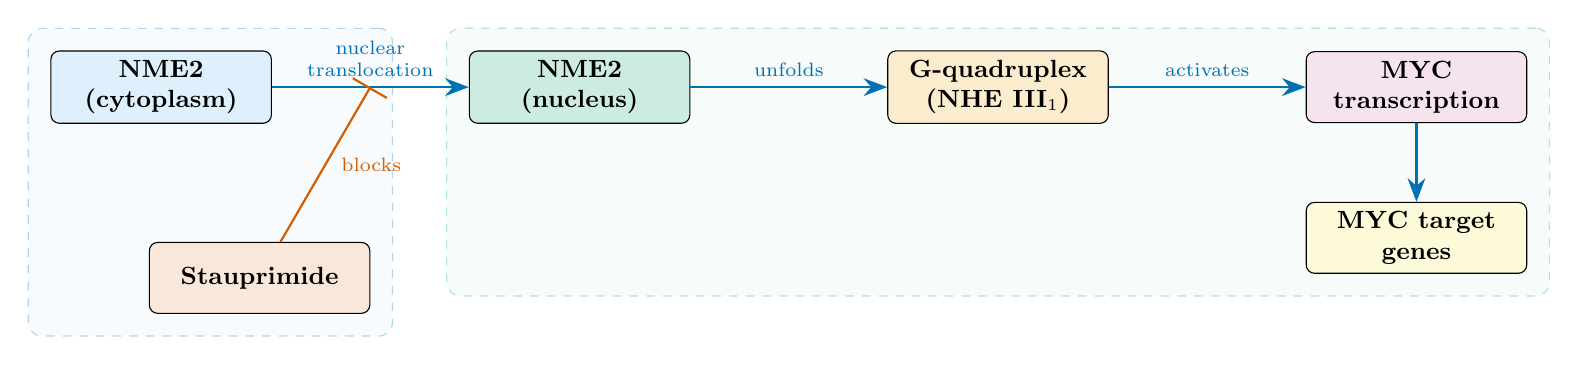
\begin{tikzpicture}[
    node distance=1.2cm and 2.0cm,
    box/.style={rectangle, draw, rounded corners=3pt, minimum width=2.8cm, minimum height=0.9cm, align=center, font=\small\bfseries},
    arrow/.style={-{Stealth[length=3mm]}, thick},
    label/.style={font=\scriptsize, align=center},
    inhibit/.style={-{Bar[width=5mm]}, thick, cbVermillion}
]

% Cytoplasm region
\node[box, fill=cbSkyBlue!20] (nme2cyto) {NME2\\(cytoplasm)};
\node[box, fill=cbGreen!20, right=2.5cm of nme2cyto] (nme2nuc) {NME2\\(nucleus)};
\node[box, fill=cbOrange!20, right=2.5cm of nme2nuc] (gquad) {G-quadruplex\\(NHE III$_1$)};
\node[box, fill=cbPurple!20, right=2.5cm of gquad] (myc) {MYC\\transcription};

% Arrows
\draw[arrow, cbBlue] (nme2cyto) -- node[above, label] {nuclear\\translocation} (nme2nuc);
\draw[arrow, cbBlue] (nme2nuc) -- node[above, label] {unfolds} (gquad);
\draw[arrow, cbBlue] (gquad) -- node[above, label] {activates} (myc);

% Stauprimide inhibition
\node[box, fill=cbVermillion!15, below=1.5cm of nme2cyto, xshift=1.25cm] (staup) {Stauprimide};
\draw[inhibit] (staup) -- node[right, label, xshift=2pt] {blocks} ($(nme2cyto)!0.5!(nme2nuc)$);

% Downstream
\node[box, fill=cbYellow!20, below=1.0cm of myc] (targets) {MYC target\\genes};
\draw[arrow, cbBlue] (myc) -- (targets);

% Region labels
\begin{scope}[on background layer]
\node[draw=cbBlue!30, dashed, fill=cbBlue!3, rounded corners=5pt, fit=(nme2cyto)(staup), inner sep=8pt, label={[font=\scriptsize\itshape]above:Cytoplasm}] {};
\node[draw=cbGreen!30, dashed, fill=cbGreen!3, rounded corners=5pt, fit=(nme2nuc)(gquad)(myc)(targets), inner sep=8pt, label={[font=\scriptsize\itshape]above:Nucleus}] {};
\end{scope}

\end{tikzpicture}
\caption{\textbf{The NME2-MYC transcriptional axis and stauprimide intervention.} NME2 translocates from the cytoplasm to the nucleus, where it binds and unfolds the G-quadruplex structure in the NHE~III$_1$ element of the MYC promoter, activating MYC transcription and downstream target gene expression. Stauprimide binds NME2 and blocks its nuclear translocation, maintaining the G-quadruplex in its folded (silencing) conformation.
\emph{Data source:} Mechanism based on Bouvard et al.~\cite{bouvard2017} and Thakur et al.~\cite{thakur2009}.}
\label{fig:pathway}
\end{figure}

\section{Stauprimide: Mechanism of Action}

Stauprimide is a semi-synthetic indolocarbazole structurally related to staurosporine. Despite this structural similarity, stauprimide does not function as a broad-spectrum kinase inhibitor~\cite{bouvard2017}. Its mechanism of action is mechanistically distinct: stauprimide binds NME2 and specifically prevents its nuclear translocation without affecting NME2 kinase activity, total protein levels, or mRNA expression~\cite{bouvard2017,zhu2009}. Treatment with stauprimide at 5~$\mu$M for 3~hours significantly reduces nuclear NME2 levels while leaving cytoplasmic NME2 unchanged, as demonstrated by nuclear--cytosolic fractionation and immunostaining~\cite{bouvard2017}.

The functional consequence of NME2 cytoplasmic retention is rapid and selective suppression of MYC transcription. In RXF~393 renal cancer cells, stauprimide reduces MYC mRNA levels with an EC$_{50}$ of 610~$\pm$~90~nM, with a consistent approximately 40\% reduction maintained across 6, 12, and 24~hour timepoints~\cite{bouvard2017}. Sensitivity varies across cell lines in a context-dependent manner: KG1A leukemia cells exhibit an EC$_{50}$ of 400~$\pm$~50~nM with up to 90\% maximal suppression, while CAKI-1 renal cells show an EC$_{50}$ of 1,004~$\pm$~142~nM~\cite{bouvard2017}. Across a broader panel of cancer cell lines spanning breast, melanoma, prostate, hepatoma, colorectal, lung, and pancreatic origins, EC$_{50}$ values range from 30~nM to 8~$\mu$M~\cite{bouvard2017}.

% ---- Figure 2: EC50 Bar Chart ----
\begin{figure}[htbp]
\centering
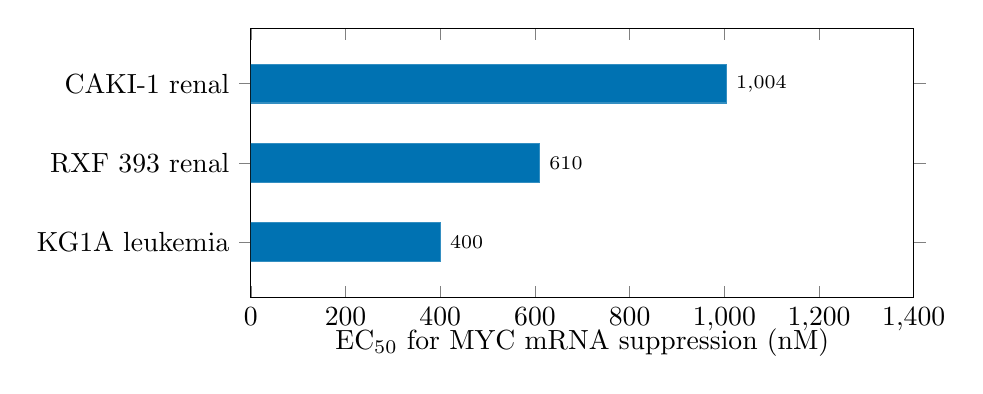
\begin{tikzpicture}
\begin{axis}[
    xbar,
    width=10cm, height=5cm,
    xlabel={EC$_{50}$ for MYC mRNA suppression (nM)},
    symbolic y coords={{KG1A leukemia}, {RXF 393 renal}, {CAKI-1 renal}},
    ytick=data,
    xmin=0, xmax=1400,
    nodes near coords,
    nodes near coords align={horizontal},
    every node near coord/.append style={font=\scriptsize},
    bar width=14pt,
    enlarge y limits=0.35,
    ylabel={},
    title={},
    cycle list={
        {fill=cbBlue, draw=cbBlue!80},
        {fill=cbVermillion, draw=cbVermillion!80},
        {fill=cbGreen, draw=cbGreen!80}
    },
    every axis x label/.style={at={(axis description cs:0.5,-0.08)}, anchor=north},
]
\addplot coordinates {(400,{KG1A leukemia}) (610,{RXF 393 renal}) (1004,{CAKI-1 renal})};
\end{axis}
\end{tikzpicture}
\caption{\textbf{Stauprimide EC$_{50}$ values for MYC mRNA suppression across cancer cell lines.} Horizontal bars show the concentration of stauprimide required to achieve 50\% suppression of MYC mRNA, as measured by qRT-PCR at 24~hours. Values represent mean $\pm$ SEM from the reported dose-response curves. Across a broader panel of cancer cell lines, EC$_{50}$ values ranged from 30~nM to 8~$\mu$M depending on cellular context.
\emph{Data source:} Bouvard et al.~\cite{bouvard2017}, reported values only; no interpolated data.}
\label{fig:ec50}
\end{figure}

Stauprimide demonstrates favorable pharmacokinetic properties for in vivo use. Oral administration at 20~mg/kg achieves a maximum plasma concentration (C$_{\text{max}}$) of 1.85--2.09~$\mu$M, comparable to the in vitro active range, with a half-life of approximately 4~hours~\cite{bouvard2017}. At a therapeutic dose of 50~mg/kg orally once daily, stauprimide is well tolerated in mice with no adverse effects on body weight, motor function, or plasma chemistry~\cite{bouvard2017}. In xenograft models, this dose achieves tumor drug concentrations of 1.8--3.6~$\mu$M, exceeding the cellular EC$_{50}$ values, and almost completely blocks tumor growth in both RXF~393 ($n$~=~10/group, $P$~$<$~0.001) and CAKI-1 ($n$~=~5/group, $P$~$<$~0.05) models~\cite{bouvard2017}. Immunohistochemistry confirmed reduced MYC protein in treated tumors, and qRT-PCR verified suppression of MYC transcription in tumor tissue~\cite{bouvard2017}.

Despite these promising results, the precise binding site of stauprimide on NME2 has not been determined. No co-crystal structure of the stauprimide--NME2 complex has been published, and the structural basis for selectivity over NME1 remains an open question. The original identification by Zhu and colleagues used affinity-based methods to establish NME2 as the target~\cite{zhu2009}, but detailed binding kinetics (K$_d$ values) were not reported in either the stem cell or cancer context.

\section{NDPK Hexamer Dynamics: A New Structural Framework}

Nucleoside diphosphate kinases of group~I (NME1, NME2, NME3, NME4) are evolutionarily conserved enzymes that assemble into hexamers with D3 symmetry, organized as a bilayer of two stacked trimers~\cite{boissan2018,karlsson1996}. NME1 and NME2 are the most abundant cytosolic isoforms and share 88\% amino acid sequence identity, differing at approximately 18~residue positions~\cite{gilles1991}. Despite this high similarity, the two isoforms have distinct isoelectric points (NME1 acidic, NME2 basic), different surface charge distributions, and partially non-overlapping cellular functions~\cite{lim2024,puts2018}.

Lim and Natarajan recently performed the first systematic computational analysis of human NDPK hexamer assembly, stability, and dynamics~\cite{lim2024}. Using crystal structures from the Protein Data Bank (NME1: PDB 1JXV; NME2: PDB 8PYW; NME3: PDB 1ZS6; NME4: PDB 1EHW), they conducted 200~ns molecular dynamics simulations with the AMBER24 force field (ff14SB) and calculated binding free energies using the MM/GBSA method. Their findings establish several principles relevant to understanding stauprimide's mechanism.

First, the conserved Arg27 residue (NME1/2 numbering) is critical for hexameric assembly across all group~I NDPKs. Single arginine-to-alanine mutations destabilize the hexamer without causing complete disassembly, while combined mutations---particularly in NME4, which has a shorter C-terminal region---can drive the hexamer-to-dimer transition~\cite{lim2024}.

Second, the C-terminal tail (approximately 10~residues) is essential for hexamer stability. It makes intermolecular contacts with the Kpn loop (residues 94--114) of an adjacent monomer, burying approximately 300~\AA$^2$ of surface area at the trimer interface. Truncation of the C-terminal 10~residues ($\Delta$10ct) dramatically destabilizes hexamers: the binding free energy of the NME2 homohexamer shifts from $-$163.75~$\pm$~1.68 to $-$92.65~$\pm$~1.50~kcal/mol upon truncation, a destabilization of +71.10~kcal/mol~\cite{lim2024}.

Third, the Kpn loop dynamics differ significantly between NME1 and NME2. NME1 exhibits increased root mean square fluctuation (RMSF) in residues 54--57 and 94--98, forming a flexible ``clamp'' that facilitates ligand accessibility to the active site cleft. By contrast, NME2 shows a more rigid Kpn loop, which restricts active site access but exposes positively charged surface residues important for DNA recognition~\cite{lim2024,tossounian2023}.

% ---- Figure 3: Binding Free Energies ----
\begin{figure}[htbp]
\centering
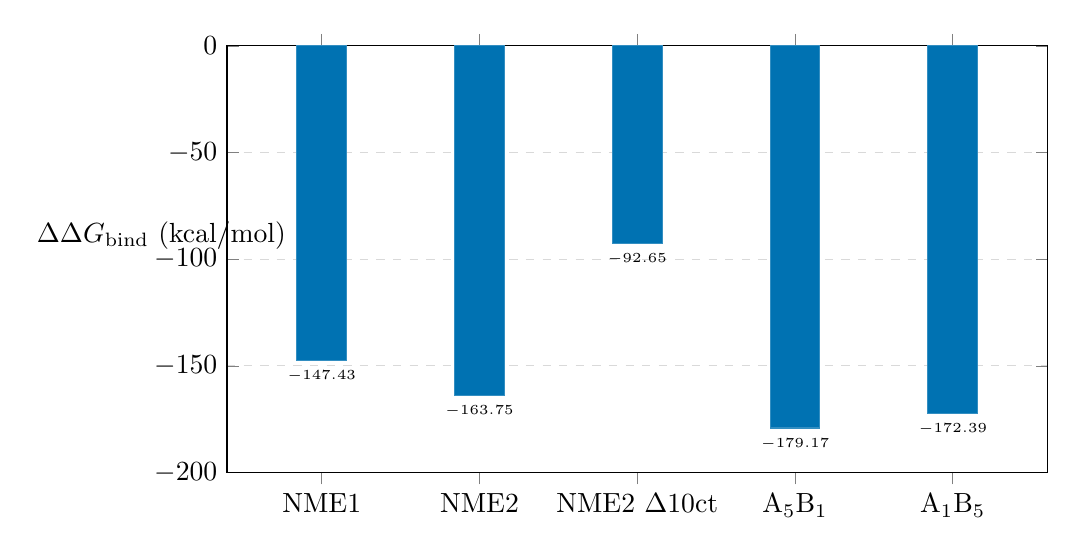
\begin{tikzpicture}
\begin{axis}[
    ybar,
    width=12cm, height=7cm,
    ylabel={$\Delta\Delta G_{\text{bind}}$ (kcal/mol)},
    symbolic x coords={NME1, NME2, NME2 $\Delta$10ct, A$_5$B$_1$, A$_1$B$_5$},
    xtick=data,
    ymin=-200, ymax=0,
    bar width=18pt,
    enlarge x limits=0.15,
    nodes near coords,
    nodes near coords align={vertical},
    every node near coord/.append style={font=\tiny, rotate=0},
    legend style={at={(0.98,0.98)}, anchor=north east, font=\small},
    ymajorgrids=true,
    grid style={dashed, gray!30},
    cycle list={
        {fill=cbBlue, draw=cbBlue!80},
    },
    every axis y label/.style={at={(axis description cs:-0.08,0.5)}, anchor=south},
]
\addplot coordinates {
    (NME1, -147.43)
    (NME2, -163.75)
    (NME2 $\Delta$10ct, -92.65)
    (A$_5$B$_1$, -179.17)
    (A$_1$B$_5$, -172.39)
};
\end{axis}
\end{tikzpicture}
\caption{\textbf{Binding free energies of NDPK hexamer configurations.} MM/GBSA-calculated binding free energies ($\Delta\Delta G_{\text{bind}}$) for NME1 and NME2 homohexamers, C-terminally truncated NME2 ($\Delta$10ct), and the two most stable NME1-NME2 heterohexamer configurations (A$_5$B$_1$: five NME1 + one NME2; A$_1$B$_5$: one NME1 + five NME2). More negative values indicate greater thermodynamic stability. The A$_5$B$_1$ and A$_1$B$_5$ penta-monomer configurations exceed both homohexamers in stability. C-terminal truncation destabilizes NME2 by +71.10~kcal/mol.
\emph{Data source:} Lim \& Natarajan~\cite{lim2024}, Tables~1 and~3.}
\label{fig:energy}
\end{figure}

Fourth, and most relevant to the stauprimide question, NME1-NME2 heterohexamers are more stable than either homohexamer. Lim and Natarajan systematically modeled all 47~possible heterohexamer configurations (reduced to 11~non-redundant by symmetry) and found that penta-monomer configurations dominate: the A$_5$B$_1$ complex (five NME1, one NME2) has a $\Delta\Delta G_{\text{bind}}$ of $-$179.17~$\pm$~3.29~kcal/mol, and the A$_1$B$_5$ complex (one NME1, five NME2) has $-$172.39~$\pm$~1.99~kcal/mol, compared to $-$147.43~$\pm$~1.90 for the NME1 homohexamer and $-$163.75~$\pm$~1.68 for the NME2 homohexamer~\cite{lim2024}. The A$_1$B$_5$ configuration is proposed as the predominant nuclear species based on the higher nuclear abundance of NME2 and the greater stability of NME2-enriched configurations~\cite{lim2024}.

% ---- Table 1: Heterohexamer Configurations ----
\begin{table}[htbp]
\centering
\caption{\textbf{Selected NME1-NME2 heterohexamer binding free energies.} All values calculated by MM/GBSA from 200~ns MD trajectories. Configurations are designated by the number of NME1 (A) and NME2 (B) subunits. More negative values indicate greater stability.}
\label{tab:heterohex}
\begin{tabular}{@{}llr@{}}
\toprule
\textbf{Configuration} & \textbf{Composition} & \textbf{$\Delta\Delta G_{\text{bind}}$ (kcal/mol)} \\
\midrule
A$_6$B$_0$ & NME1 homohexamer & $-$147.43 $\pm$ 1.90 \\
A$_0$B$_6$ & NME2 homohexamer & $-$163.75 $\pm$ 1.68 \\
\addlinespace
A$_5$B$_1$ (pentamer) & 5 NME1 + 1 NME2 & $-$179.17 $\pm$ 3.29 \\
A$_1$B$_5$ (pentamer) & 1 NME1 + 5 NME2 & $-$172.39 $\pm$ 1.99 \\
A$_3$B$_3$ (C$_{10}$) & 3 NME1 + 3 NME2 & $-$168.47 $\pm$ 1.95 \\
A$_2$B$_4$ (B$_{10}$) & 2 NME1 + 4 NME2 & $-$169.28 $\pm$ 2.26 \\
A$_3$B$_3$ (D$_5$) & 3 NME1 + 3 NME2 & $-$142.09 $\pm$ 1.68 \\
\bottomrule
\end{tabular}

\smallskip
{\footnotesize \emph{Data source:} Reproduced from Lim \& Natarajan~\cite{lim2024}, Tables~1 and~3. All values are from computational analysis; no experimental measurements.}
\end{table}

A key structural finding is that the approximately 18~amino acid positions differing between NME1 and NME2 are located outside the hexameric intersubunit interface. This means that heterohexamers of any composition are structurally nearly indistinguishable at the interface level, yet their surface properties differ, potentially enabling distinct protein--protein and protein--DNA interactions depending on subunit composition~\cite{lim2024}.

\section{Integrative Analysis: A Proposed Structural Mechanism}

\noindent\fcolorbox{cbOrange}{hypothesisbg}{%
\parbox{\dimexpr\linewidth-2\fboxsep-2\fboxrule}{%
\textbf{Note:} The following section presents a \textbf{hypothesis} derived from integration of published data. No original experimental or computational data supporting this model have been generated. This hypothesis requires validation through structural biology and biophysical approaches.}}

\bigskip

The convergence of stauprimide pharmacology and NDPK hexamer dynamics suggests a mechanistic model in which stauprimide acts as an ``oligomer-selective'' inhibitor---not by blocking enzymatic activity or DNA binding directly, but by preventing the assembly of the specific oligomeric species required for nuclear translocation.

We propose that stauprimide binds NME2 at or near the approximately 18 isoform-specific residues that distinguish it from NME1. Because these residues are located outside the hexameric interface~\cite{lim2024}, they are solvent-exposed and accessible to small molecules without requiring disruption of existing hexameric contacts. Binding at these positions could exert its effect through at least two non-mutually exclusive mechanisms.

First, stauprimide binding may propagate conformational changes to the nearby Kpn loop (residues 94--114). NME2 already exhibits a more rigid Kpn loop than NME1~\cite{lim2024}; drug binding could further constrain this loop, locking NME2 monomers in a conformation incompatible with the adaptive changes required for heterohexamer assembly. The C-terminal tail of one monomer must thread through and interact with the Kpn loop of its neighbor to stabilize the trimer interface~\cite{vieira2015,lim2024}. If stauprimide rigidifies this region, the energetically favorable A$_1$B$_5$ assembly would be disrupted.

Second, stauprimide binding could mask surface features required for nuclear import recognition. The NME1-NME2 heterohexamer may present a specific surface topology---distinct from either homohexamer---that is recognized by nuclear import machinery. By altering the conformation or electrostatic properties of NME2's isoform-specific surface, stauprimide could prevent the formation of this recognition-competent surface without affecting NME2 protein levels or catalytic function, consistent with the observed pharmacology~\cite{bouvard2017}.

This model explains two key observations: (1)~the selectivity of stauprimide for NME2 over NME1, which arises from binding at isoform-specific residue positions that are structurally distinct between the two proteins; and (2)~the cytoplasmic retention phenotype without kinase inhibition, which arises from disruption of oligomeric assembly rather than active site blockade. The model also predicts that stauprimide would preferentially disrupt heterohexameric species over NME2 homohexamers, as the A$_1$B$_5$ configuration involves more extensive NME2--NME1 interfaces at which conformational perturbation could propagate.

\section{Clinical Implications and Therapeutic Landscape}

The NME2-MYC transcriptional axis has recently gained clinical significance in the context of treatment resistance. Panja and colleagues reconstructed a CRPC-specific regulatory network and identified NME2 as an upstream activator of MYC in enzalutamide-resistant prostate cancer~\cite{panja2024}. Their analysis of clinical data revealed that patients with elevated NME2-MYC co-expression were five-fold less likely to benefit from enzalutamide, and that NME2 and MYC levels could increase in response to enzalutamide exposure, suggesting an adaptive resistance mechanism~\cite{panja2024}. Therapeutic targeting of MYC with the small-molecule MYC inhibitor MYCi975, combined with NME2 knockdown, reversed enzalutamide resistance in preclinical models~\cite{panja2024}. These findings suggest that stauprimide or optimized analogs could serve as components of combination strategies to overcome treatment resistance in CRPC.

% ---- Table 2: Comparison of MYC-Targeting Strategies ----
\begin{table}[htbp]
\centering
\caption{\textbf{Comparison of therapeutic strategies for indirect MYC suppression.} Each approach targets a different node in MYC transcriptional regulation. Selectivity, mechanism, and limitations differ substantially.}
\label{tab:strategies}
\begin{tabular}{@{}p{2.5cm}p{3.0cm}p{3.5cm}p{3.5cm}@{}}
\toprule
\textbf{Strategy} & \textbf{Mechanism} & \textbf{Selectivity} & \textbf{Limitations} \\
\midrule
Stauprimide (NME2 inhibitor) & Blocks NME2 nuclear translocation & Selective for MYC targets (GSEA: 2/50 gene sets) & No co-crystal structure; requires wild-type NHE~III$_1$ \\
\addlinespace
BET inhibitors (e.g., JQ1) & Disrupts epigenetic MYC activation & Broad transcriptional effects & Affects genes beyond MYC; resistance emerges \\
\addlinespace
G-quadruplex stabilizers & Maintains silencing structure in MYC promoter & Variable G4 selectivity & Off-target effects on other G4-containing promoters \\
\addlinespace
MYC--MAX disruptors & Prevents MYC--MAX dimerization & Direct MYC targeting & Large interaction surface; low potency \\
\bottomrule
\end{tabular}

\smallskip
{\footnotesize \emph{Data sources:} Bouvard et al.~\cite{bouvard2017} for stauprimide; Delmore et al.~\cite{delmore2011} for BET inhibitors; Siddiqui-Jain et al.~\cite{siddiquijain2002} for G-quadruplex stabilizers.}
\end{table}

The broader therapeutic landscape for targeting NME heterooligomerization was outlined by Abu-Taha and colleagues, who proposed that peptides or small molecules disrupting specific NME interaction sites could offer novel therapeutic approaches~\cite{abutaha2018}. The structural framework from Lim and Natarajan now provides the computational foundation for rational design of such interventions~\cite{lim2024}.

NME2-targeting approaches offer a potential advantage over direct MYC inhibitors in the context of immuno-oncology. MYC directly upregulates immune checkpoint molecules CD47 and PD-L1~\cite{casey2016}; suppression of MYC through NME2 inhibition could therefore sensitize tumors to immune surveillance. Notably, stauprimide is effective in both human and murine cancer cells at comparable concentrations~\cite{bouvard2017}, enabling investigation in syngeneic mouse models with intact immune systems---a significant advantage over xenograft systems for studying immunomodulatory effects.

\section{Future Directions and Open Questions}

Several critical experiments are required to validate the structural hypothesis proposed in this perspective and to advance NME2-targeting therapeutics toward clinical application.

The most pressing need is a co-crystal structure of stauprimide bound to NME2. X-ray crystallography or cryo-electron microscopy of the stauprimide--NME2 complex would directly reveal the binding site, the conformational changes induced by drug binding, and whether stauprimide contacts isoform-specific residues as hypothesized. In the absence of experimental structures, molecular dynamics simulations of stauprimide docked to the NME2 monomer and to the A$_1$B$_5$ heterohexamer could provide preliminary structural predictions, building on the computational framework established by Lim and Natarajan~\cite{lim2024}.

Structure--activity relationship (SAR) studies of stauprimide analogs represent another critical gap. The Bouvard study explicitly called for ``further development of stauprimide through medicinal chemistry efforts to afford more potent analogs''~\cite{bouvard2017}, yet no published SAR campaign has been reported as of this writing. Systematic modification of the indolocarbazole scaffold, guided by knowledge of the NME2 binding site, could yield compounds with improved potency, selectivity, and pharmacokinetic properties.

The clinical relevance of the A$_1$B$_5$ heterohexamer model should be evaluated experimentally. Native mass spectrometry and crosslinking mass spectrometry of endogenous NME1-NME2 complexes from nuclear and cytoplasmic fractions could determine whether the predicted penta-monomer configurations exist in vivo and whether stauprimide treatment shifts the oligomeric distribution.

Given the findings of Panja and colleagues~\cite{panja2024}, stauprimide should be tested in enzalutamide-resistant CRPC models, either alone or in combination with direct MYC inhibitors such as MYCi975 or with enzalutamide retreatment. NME2-MYC co-expression could be developed as a predictive biomarker for patient stratification.

Finally, the role of NME family members beyond NME1 and NME2 warrants investigation. Recent work on NME3 in mitophagy~\cite{chen2024} and NME4 in mitochondrial function~\cite{boissan2018} highlights the functional diversity of the NME superfamily. Understanding whether stauprimide analogs could be designed with selectivity profiles targeting specific NME family members or heterohexamer configurations would open new therapeutic avenues.

% ---- Figure 4: Proposed Mechanism Schematic ----
\begin{figure}[htbp]
\centering
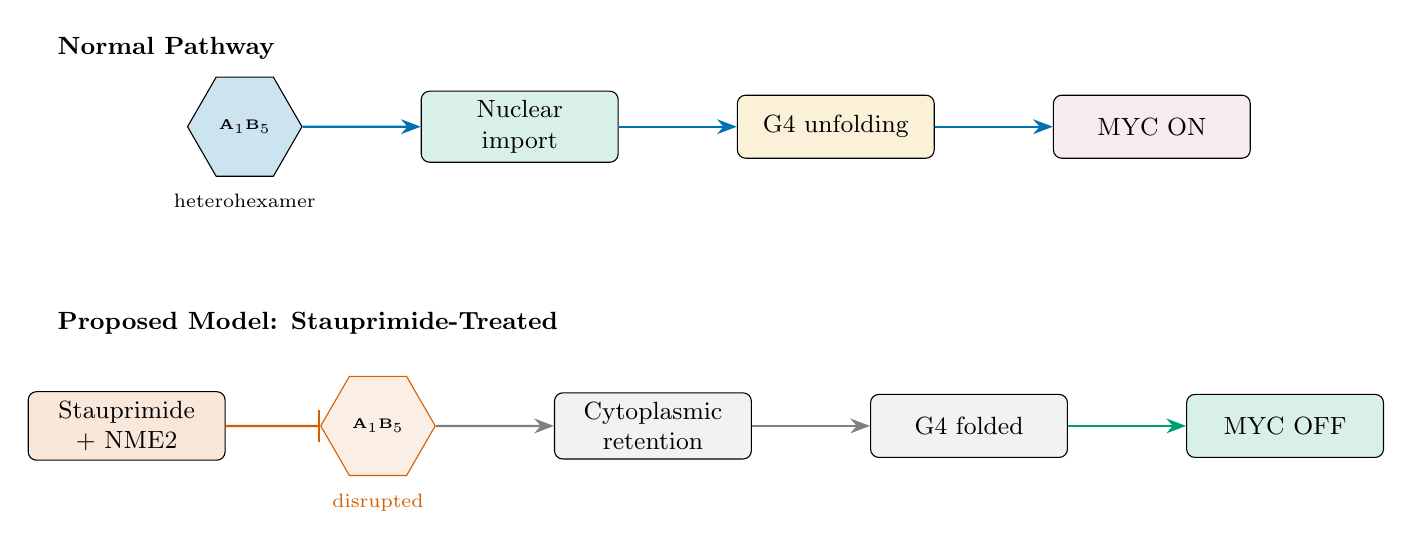
\begin{tikzpicture}[
    node distance=0.8cm and 1.5cm,
    box/.style={rectangle, draw, rounded corners=3pt, minimum width=2.5cm, minimum height=0.8cm, align=center, font=\small},
    hexbox/.style={regular polygon, regular polygon sides=6, draw, minimum size=1.2cm, font=\tiny\bfseries},
    arrow/.style={-{Stealth[length=2.5mm]}, thick},
    inhibit/.style={-{Bar[width=4mm]}, thick, cbVermillion},
    label/.style={font=\scriptsize, align=center}
]

% Normal pathway (top row)
\node[font=\small\bfseries, anchor=west] at (-1,3.0) {\textsc{Normal Pathway}};

\node[hexbox, fill=cbBlue!20] (hex1) at (1.5,2) {A$_1$B$_5$};
\node[label, below=0.1cm of hex1] {heterohexamer};
\node[box, fill=cbGreen!15, right=1.5cm of hex1] (nuc1) {Nuclear\\import};
\node[box, fill=cbOrange!15, right=1.5cm of nuc1] (gq1) {G4 unfolding};
\node[box, fill=cbPurple!15, right=1.5cm of gq1] (myc1) {MYC ON};

\draw[arrow, cbBlue] (hex1) -- (nuc1);
\draw[arrow, cbBlue] (nuc1) -- (gq1);
\draw[arrow, cbBlue] (gq1) -- (myc1);

% Stauprimide pathway (bottom row)
\node[font=\small\bfseries, anchor=west] at (-1,-0.5) {\textsc{Proposed Model: Stauprimide-Treated}};

\node[box, fill=cbVermillion!15] (staup2) at (0,-1.8) {Stauprimide\\+ NME2};
\node[hexbox, fill=cbVermillion!10, draw=cbVermillion, right=1.2cm of staup2] (hex2) {A$_1$B$_5$};
\node[label, below=0.1cm of hex2] {\color{cbVermillion}disrupted};
\draw[inhibit] (staup2) -- (hex2);

\node[box, fill=gray!10, right=1.5cm of hex2] (cyt2) {Cytoplasmic\\retention};
\node[box, fill=gray!10, right=1.5cm of cyt2] (gq2) {G4 folded};
\node[box, fill=cbGreen!15, right=1.5cm of gq2] (myc2) {MYC OFF};

\draw[arrow, gray] (hex2) -- (cyt2);
\draw[arrow, gray] (cyt2) -- (gq2);
\draw[arrow, cbGreen] (gq2) -- (myc2);

\end{tikzpicture}
\caption{\textbf{Proposed model for stauprimide-mediated MYC suppression via heterohexamer disruption.} \textit{Top:} Under normal conditions, NME1-NME2 A$_1$B$_5$ heterohexamers assemble, translocate to the nucleus, unfold the G-quadruplex in the MYC promoter, and activate transcription. \textit{Bottom:} Stauprimide binds NME2 and disrupts A$_1$B$_5$ assembly, leading to cytoplasmic retention of NME2, maintained G-quadruplex silencing, and MYC suppression. \textbf{This is a proposed model requiring experimental validation.}
\emph{Hypothesis based on integration of:} Bouvard et al.~\cite{bouvard2017} and Lim \& Natarajan~\cite{lim2024}.}
\label{fig:model}
\end{figure}

\section{Conclusion}

The NME2-MYC transcriptional axis represents a mechanistically validated and clinically relevant target for cancer therapy. Stauprimide provides proof-of-concept that pharmacological inhibition of NME2 nuclear translocation can selectively suppress MYC transcription with favorable selectivity and in vivo efficacy. The recent elucidation of NDPK hexamer dynamics by Lim and Natarajan offers the first structural framework for understanding how NME oligomerization governs nuclear competence, and identifies the A$_1$B$_5$ heterohexamer as a potential molecular target.

We propose that stauprimide acts by disrupting this heterohexameric assembly through binding at NME2's isoform-specific surface residues, a hypothesis that makes specific and testable predictions about the drug's binding site, conformational effects, and oligomeric selectivity. Validation of this model through co-crystallography, SAR studies, and testing in drug-resistant cancer models would provide the foundation for rational development of next-generation NME2-targeting therapeutics. Given the convergence of MYC's role in treatment resistance, immune evasion, and NME2's position as a druggable upstream regulator, this axis merits sustained investigation.

\section*{Data Availability}

This perspective article synthesizes published data from the cited references. No original experimental or computational datasets were generated. The source data for all figures and tables are from Bouvard et al.~\cite{bouvard2017} and Lim \& Natarajan~\cite{lim2024} and are available in the respective publications and their supplementary materials.

\section*{Competing Interests}

The author declares no competing interests.

\begin{thebibliography}{19}

\bibitem{bouvard2017}
Bouvard, C., Lim, S.M., Ludka, J., Yazdani, N., Woods, A.K., Chatterjee, A.K., Schultz, P.G. \& Zhu, S.
Small molecule selectively suppresses MYC transcription in cancer cells.
\textit{Proc. Natl. Acad. Sci. USA} \textbf{114}, 3497--3502 (2017).
\href{https://doi.org/10.1073/pnas.1702663114}{doi:10.1073/pnas.1702663114}

\bibitem{lim2024}
Lim, Y.Y. \& Natarajan, K.N.
Modelling dynamics of human NDPK hexamer structure, stability and interactions.
\textit{bioRxiv} 2024.09.19.613900 (2024). [Preprint, not peer-reviewed in journal as of Feb 2026.]
\href{https://doi.org/10.1101/2024.09.19.613900}{doi:10.1101/2024.09.19.613900}

\bibitem{panja2024}
Panja, S. et al.
Mechanism-centric regulatory network identifies NME2 and MYC programs as markers of Enzalutamide resistance in CRPC.
\textit{Nat. Commun.} \textbf{15}, 352 (2024).
\href{https://doi.org/10.1038/s41467-024-44686-5}{doi:10.1038/s41467-024-44686-5}

\bibitem{zhu2009}
Zhu, S. et al.
A small molecule primes embryonic stem cells for differentiation.
\textit{Cell Stem Cell} \textbf{4}, 416--426 (2009).
\href{https://doi.org/10.1016/j.stem.2009.04.001}{doi:10.1016/j.stem.2009.04.001}

\bibitem{abutaha2018}
Abu-Taha, I.H., Vettel, C. \& Wieland, T.
Targeting altered Nme heterooligomerization in disease?
\textit{Oncotarget} \textbf{9}, 1492--1493 (2018).
\href{https://doi.org/10.18632/oncotarget.22716}{doi:10.18632/oncotarget.22716}

\bibitem{thakur2009}
Thakur, R.K. et al.
Metastases suppressor NM23-H2 interaction with G-quadruplex DNA within c-MYC promoter nuclease hypersensitive element induces c-MYC expression.
\textit{Nucleic Acids Res.} \textbf{37}, 172--183 (2009).
\href{https://doi.org/10.1093/nar/gkn919}{doi:10.1093/nar/gkn919}

\bibitem{postel1996}
Postel, E.H., Berberich, S.J., Flint, S.J. \& Ferrone, C.A.
Mutational analysis of NM23-H2/NDP kinase identifies the structural domains critical to recognition of a c-myc regulatory element.
\textit{Proc. Natl. Acad. Sci. USA} \textbf{93}, 6892--6897 (1996).
\href{https://doi.org/10.1073/pnas.93.14.6892}{doi:10.1073/pnas.93.14.6892}

\bibitem{siddiquijain2002}
Siddiqui-Jain, A., Grand, C.L., Bearss, D.J. \& Hurley, L.H.
Direct evidence for a G-quadruplex in a promoter region and its targeting with a small molecule to repress c-MYC transcription.
\textit{Proc. Natl. Acad. Sci. USA} \textbf{99}, 11593--11598 (2002).
\href{https://doi.org/10.1073/pnas.182256799}{doi:10.1073/pnas.182256799}

\bibitem{delmore2011}
Delmore, J.E. et al.
BET bromodomain inhibition as a therapeutic strategy to target c-Myc.
\textit{Cell} \textbf{146}, 904--917 (2011).
\href{https://doi.org/10.1016/j.cell.2011.08.017}{doi:10.1016/j.cell.2011.08.017}

\bibitem{tossounian2023}
Tossounian, M.A. et al.
A unique mode of coenzyme A binding to the nucleotide binding pocket of human metastasis suppressor NME1.
\textit{Int. J. Mol. Sci.} \textbf{24}, 9359 (2023).
\href{https://doi.org/10.3390/ijms24119359}{doi:10.3390/ijms24119359}

\bibitem{vieira2015}
Vieira, P.S. et al.
The role of the C-terminus and Kpn loop in the quaternary structure stability of nucleoside diphosphate kinase from Leishmania parasites.
\textit{J. Struct. Biol.} \textbf{192}, 336--341 (2015).
\href{https://doi.org/10.1016/j.jsb.2015.09.017}{doi:10.1016/j.jsb.2015.09.017}

\bibitem{gilles1991}
Gilles, A.M. et al.
Nucleoside diphosphate kinase from human erythrocytes: structural characterization of the two polypeptide chains responsible for heterogeneity of the hexameric enzyme.
\textit{J. Biol. Chem.} \textbf{266}, 8784--8789 (1991).

\bibitem{karlsson1996}
Karlsson, A. et al.
Nucleoside diphosphate kinase: investigation of the intersubunit contacts by site-directed mutagenesis and crystallography.
\textit{J. Biol. Chem.} \textbf{271}, 19928--19934 (1996).
\href{https://doi.org/10.1074/jbc.271.33.19928}{doi:10.1074/jbc.271.33.19928}

\bibitem{boissan2018}
Boissan, M., Schlattner, U. \& Lacombe, M.L.
The NDPK/NME superfamily: state of the art.
\textit{Lab. Invest.} \textbf{98}, 164--174 (2018).
\href{https://doi.org/10.1038/labinvest.2017.137}{doi:10.1038/labinvest.2017.137}

\bibitem{casey2016}
Casey, S.C. et al.
MYC regulates the antitumor immune response through CD47 and PD-L1.
\textit{Science} \textbf{352}, 227--231 (2016).
\href{https://doi.org/10.1126/science.aac9935}{doi:10.1126/science.aac9935}

\bibitem{thakur2014}
Thakur, R.K. et al.
Non-metastatic 2 (NME2)-mediated suppression of lung cancer metastasis involves transcriptional regulation of key cell adhesion factor vinculin.
\textit{Nucleic Acids Res.} \textbf{42}, 11589--11600 (2014).
\href{https://doi.org/10.1093/nar/gku860}{doi:10.1093/nar/gku860}

\bibitem{yang2006}
Yang, D. \& Hurley, L.H.
Structure of the biologically relevant G-quadruplex in the c-MYC promoter.
\textit{Nucleosides Nucleotides Nucleic Acids} \textbf{25}, 951--968 (2006).

\bibitem{chen2024}
Chen, C.W. et al.
NME3 is a gatekeeper for DRP1-dependent mitophagy in hypoxia.
\textit{Nat. Commun.} \textbf{15}, 2264 (2024).
\href{https://doi.org/10.1038/s41467-024-46385-7}{doi:10.1038/s41467-024-46385-7}

\bibitem{puts2018}
Puts, G.S. et al.
Nuclear functions of NME proteins.
\textit{Lab. Invest.} \textbf{98}, 211--218 (2018).
\href{https://doi.org/10.1038/labinvest.2017.109}{doi:10.1038/labinvest.2017.109}

\end{thebibliography}

\end{document}
